\documentclass[10pt,a4paper]{article}
\usepackage[utf8]{inputenc}
\usepackage[english]{babel}
\usepackage{amsmath}
\usepackage{amsfonts}
\usepackage{amssymb}
\usepackage{makeidx}
\usepackage{biblatex}
\usepackage{graphicx}
\usepackage{fourier}
\usepackage[left=2cm,right=2cm,top=2cm,bottom=2cm]{geometry}
\author{Sigve Harang, Lukas Powalla}
\title{Space Physics Project , FYS3610}
\begin{document}
\maketitle
\newpage
\tableofcontents
\newpage
\section*{Introduction}
In this project we are going to analyse the ionospheric and auroral dynamics and its relation to the solar wind conditions. Furthermore, we will connect our observations to the current systems as well as the auroral activity and polar cap.  We will investigate in a specific timeslot of 24 hours.  
\section{Theory part}
In order to understand the movements and changes in the system of the earth and the sun, we want to introduce some basic concepts of space physics. 
A really important steady state picture of what is going on with respect to the earth's magnetic field, the interaction of the earth's magnetic field with the IMF and the consequences of the earth's environment (such as current flows or aurora) is the Dungey cycle. (only when IMF is southward orientated)
However, the dungey cycle is as already mentioned a steady state picture. (This means for example that the magnetic flux added to the open magnetic field lines through day side reconnection is equal to the magnetic flux subtracting from the open magnetic field lines through night side reconnection)
However, this cycle is in reality not a steady state picture. There are different phases of adding magnetic flux (growing of the polar cap), some kind of explosive expansion (subtraction of magnetic flux from the polar cap) and a recovery phase. This phenomena is called a "Auroral substorm". In addition to that, we can extract information about what is going on with the system earth-sun by looking at different data sets containing information about the magnetic field on earth, the solar wind bulk speed, the auroral intensity, the current density and further data from different physical measurements. 
Based on this measurements we will interpret the received data and relate it to the theoretical predictions and the models we introduced in the theoretical part.

\subsection{The Dungey cycle - a steady state picture}

\begin{figure}[h]
\centering
\caption{Dungey cycle}
\label{aurora substorm}
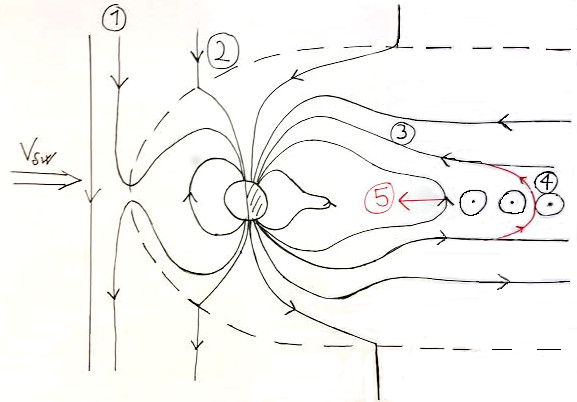
\includegraphics[scale=0.5]{solvind.jpg}
\end{figure}

If the magnetic field is northward orientated nothing happens at the boundary of the terrestrial magnetic field and the magnetic field of the sun/ the solar wind. IMF can not mix with the terrestrial magnetic field because everything in frozen in. Since the terrestrial magnetic field and the IMF are not anti-parallel orientated, magnetic reconnection does not occur and hence, everything is and stays frozen in. 
However, if the IMF is southward orientated, we do have anti-parallel orientated magnetic field at the boundary of terrestrial magnetic field and the IMF (at the magnetopause). Therefore, magnetic reconnection occurs at the magnetopause, which causes a cyclic reconnection pattern at day/night-side. If we assume a steady state picture, we call the cycle, which happens for southward IMF, the dungey cycle. The different parts of the cycle can be described as follows:
\begin{itemize}
\item[1] opposite polarity field lines reconnect at magnetopause (if IMF southward orientated
\item[2] magnetic field lines are still connected to the solar wind. (frozen in again) Therefore, the magnetic field line is draged along with the solar wind in the direction of the tale. (magnetic tension force)
\item[3] magnetic flux is added to the tail and compresses the plasma sheet (magnetic pressure increases, plasma sheet gets thinner and thinner)
\item[4] magnetic reconnection occurs in the tail. 
\item[5] reconnected magnetic field lines return to the day side (imagination of "rubber bands" help to understand this)
\end{itemize}

\subsection{Auroral substorm}
As already mentioned in the introduction, the assumption of a steady state picture is not a appropriate description of what happens in reality. To specify this, the rate of adding magnetic flux and the rate of subtracting magnetic flux from the polar cap are not equal. However, after studying data from different measurements, Akasofu could state out in 1964 different phases of a cycle so called:
\begin{itemize}
\item[1] groth phase
\item[2] expansion phase
\item[3] recovery phase
\end{itemize}
\subsubsection{groth phase}
The day side reconnection dominates and the aurora moves to lower latitudes. The auroral activity increases in the cusp and open magnetic flux is added to the polar cap. The magnetic flux, which is added due to the day side reconnection makes the tail radius increase.(because the field lines are draged tail-wards with the IMF )
\subsubsection{Expansion phase}
Sudden onset of night-side reconnection at the NENL. Sudden brightening of the night side aurora. Poleward and westward movement of the aurora (on average). It closes open magnetic flux. 
\subsubsection{recovery phase}
The night side reconnection continues at smaller rates and the auroral display quietens. Furthermore, the polar cap contracts and the magnetosphere returns to pro groth phase "equilibrium". 
\begin{figure}[h]
\centering
\caption{Auroral substorm}
\label{aurora substorm}
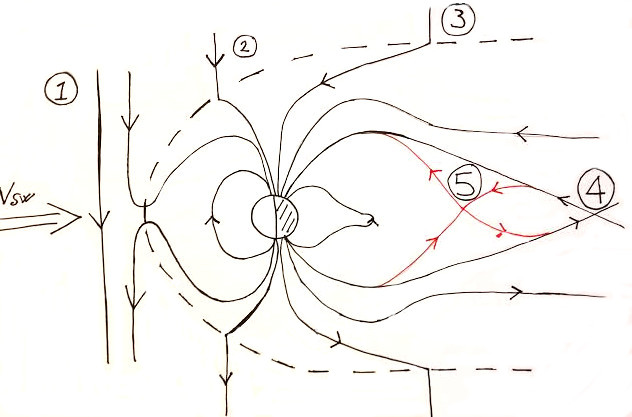
\includegraphics[scale=0.5]{solvind2.jpg}
\end{figure}

\subsection{Ionospheric currents}
\subsubsection{Petersen current, Hall current and Fieldalign currents}

\subsection{Twin cell convection}

\section{Observations}

\subsection{•}

\section{discussion}

\section{conclusion}


\section{First section}
 

\end{document}